The injection kicker magnets in the LHC are part of the injection system for the LHC machine. This system is used to match the trajectory of the injected beam to that of the stable beam path in the accelerator. An example schema for the LHC can be seen in Fig.~\ref{fig:injection-system-schema}. The system typically uses two components: a septum, which may provide a slowly rising and falling (or possibly constant), but strong, field, and kickers, which may provide a rapidly rising and falling, but comparatively weak, field to match the injected beam to the correct trajectory. Similar components are used for the fast extraction of beam (for systems such as the abort system) also.

\begin{figure}
\begin{center}
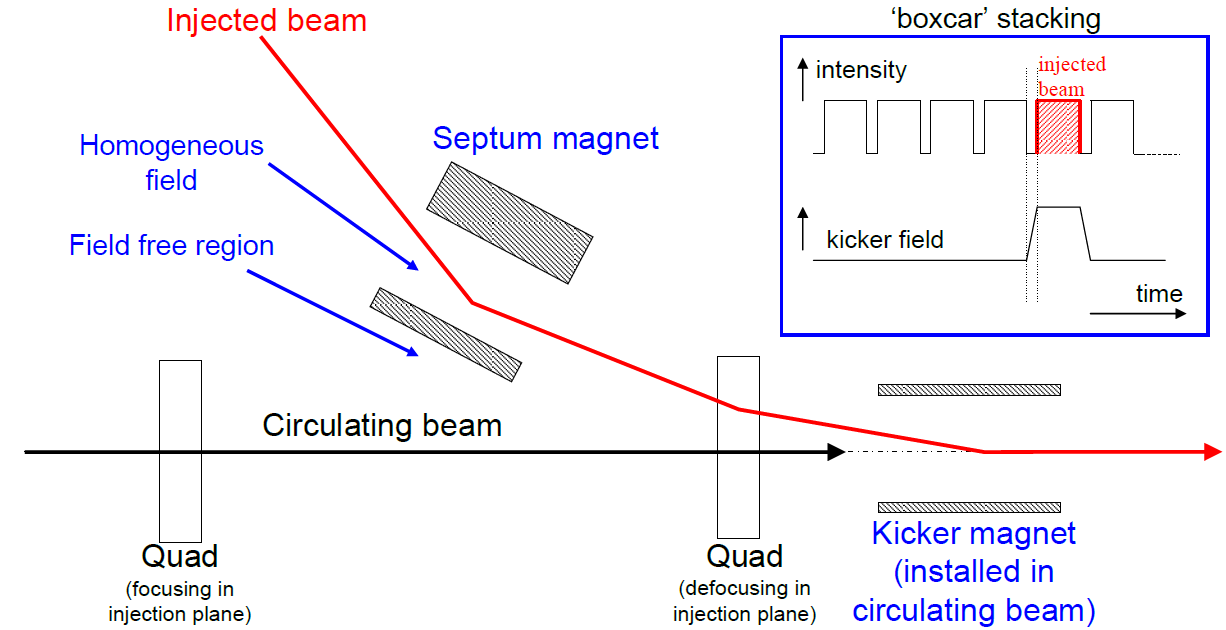
\includegraphics[width=0.6\textwidth]{LHC_MKI/figures/injection-system.png}
\end{center}
\caption{An example layout of a injection system for an accelerator. Taken from \cite{Barnes:injSys}}
\label{fig:injection-system-schema}
\end{figure}

By design kickers are generally always visible to the beam due to the need to quickly apply their kick. In order to achieve a fast field rise/fall time and field qualities desired, the yoke of the kicker magnet is usually a NiZn ferrite. In addition the need for a highly homogeneous field whilst the kick is applied, as well as the strength of the field and the costs of large aperture magnets, neccesitates that the aperture for kickers often be relatively small, meaning they are in close proximity to the beam. This leads to two concerns - that the close proximity of the beam to such a device, that may be made of either a highly lossy material \cite{Day:wireMeasFerr, Barnes:wireMeasKick, Barnes:spsKickerHeating} or a source of strong geometrical impedance \cite{Belver-Aguilar:clicStripline}, may be source of impedance that drives instabilities in the beam \cite{Salvant:spsImpModel}, and secondly that the large real component of the ferrite ferrite may be subject to intense heating in high beam current machines \cite{Barnes:spsKickerHeating}. 

\section{LHC Injection Kicker Magnets}

Each LHC injection kicker magnet (LHC-MKI, or MKI) is a 3m long travelling wave transmission line kicker magnet (ferrite length 2.7m). A transmission line magnet is a magnet that is composed of multiple cells each capacitvely coupled to ground. This means that the effective inductance that the pulse is exposed to is reduced, allowing for shorter rise times to be achieved. For LHC there are two injection regions, near IPs 2 (ALICE) and 8 (LHCb), each consisting of a septa system and four MKIs injecting vertically into the machine (the position of the LHC injection systems is shown in Fig.~\ref{fig:lhc-injection-systems}). As a transmission line magnet the magnet is constructed of a c-core ferrite yoke, segmented by alternating HV (High Voltage) and ground plates capacitively coupled together by ceramic capacitors to form a magnet of 5$\Omega$ characteristic impedance. The pulse is generated in a Pulse Forming Network (PFN) and is subsequently carried by 10 parallel coaxial cables with a total characteristic impedance of $5 \Omega$, matching the characteristic impedance of the MKI and the PFN. The performance parameters of the magnets rise time, fied strength and homogeneity are given in Tab.~\ref{tab:mki-parameters} \cite{Ducimetiere:mkiSpec}.

\begin{figure}
\begin{center}
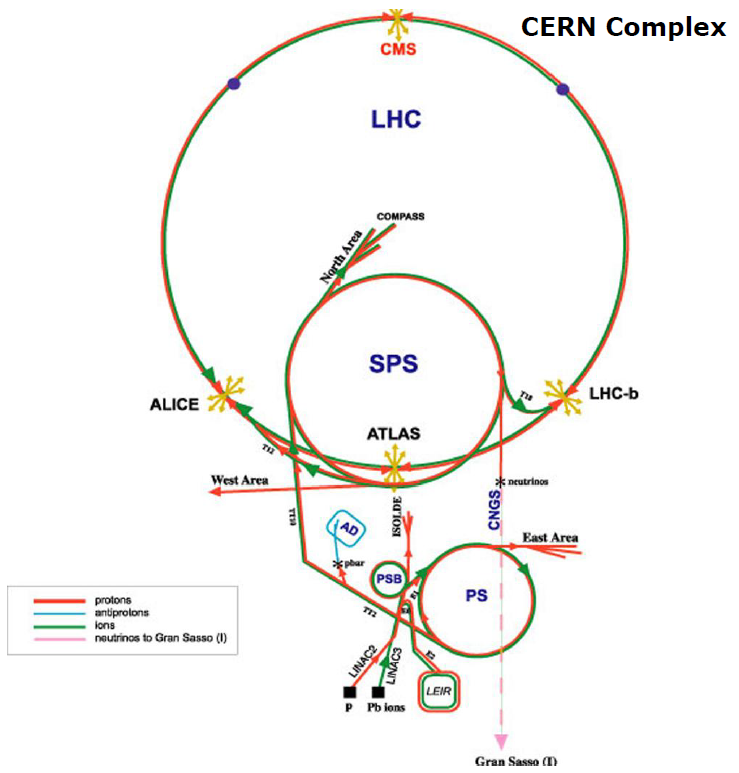
\includegraphics[width=0.75\textwidth]{LHC_MKI/figures/injection-points-lhc.png}
\end{center}
\caption{The location of the LHC injection systems in the LHC ring.}
\label{fig:lhc-injection-systems}
\end{figure}


\begin{figure}
\begin{center}
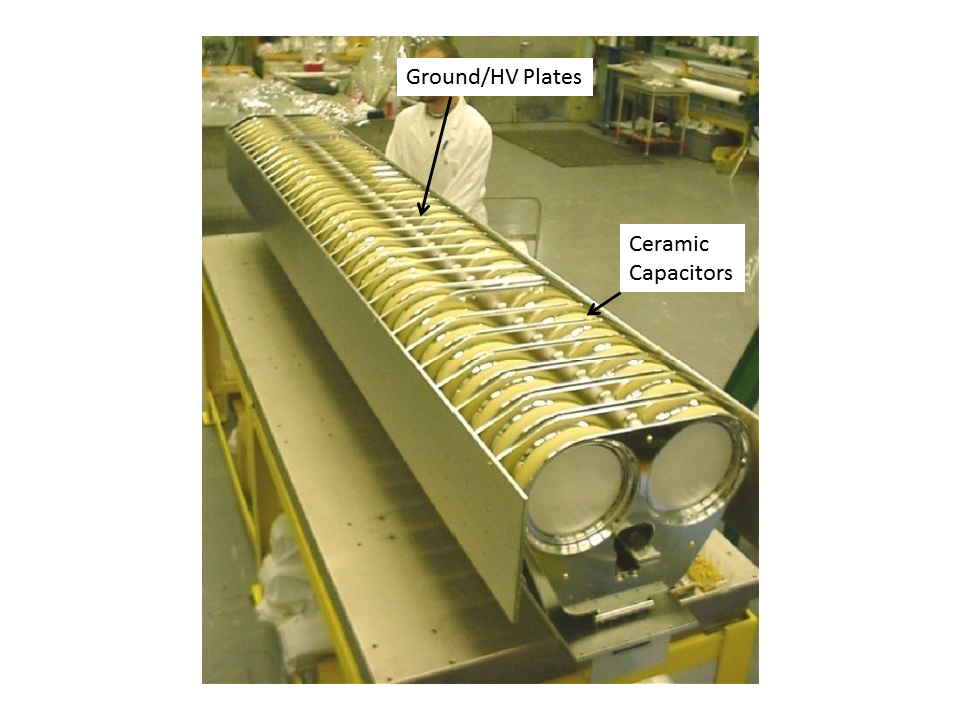
\includegraphics[height=0.4\textwidth]{LHC_MKI/figures/mki-out-vac-tank.png}
\end{center}
\caption{A cross section of an MKI. Visible are the alternating HV and ground plates, seperated by capacitor plates. The HV busbar and the ground return can be seen in the c core of the ferrite yoke.}
\label{fig:lhc-mki-cross-section}
\end{figure}

\begin{table}
\caption{MKI operational parameters}

\begin{center}
\begin{tabular}{c | c | c}
Number of Kickers per System & 4 & \\ \hline
Kick strength per magnet & 0.3 & T.m \\ \hline
Beam aperture (diameter) & 38 & mm \\ \hline
Characteristic Impedance & 5 & $\Omega$ \\ \hline
Operating charging voltage (PFN) & 54 & kV \\ \hline
Field flat top ripple & < $\pm$0.5 & \% \\ \hline
Field flat top duration & up to 7.86 & $\mu$s \\ \hline
Field rise time 0.5\%-99.5\% & 0.9 & $\mu$s \\ \hline
Field fall time 99.5\%-0.5\% & 3.0 & $\mu$s \\ \hline
Magnet kength & 2.7 & m \\ 
\end{tabular}
\end{center}
\label{tab:mki-parameters}
\end{table}